%%%%%%%%%%%%%%%%%%%%%%%%%%%%%%%%%%%%%%%
\section{Statistical Estimation Theory}
\label{sec:SDT}
%%%%%%%%%%%%%%%%%%%%%%%%%%%%%%%%%%%%%%%

% Once we have faced some of the main concepts involved in estimation problems, we are ready to formalize the problem for a general case.


%%%%%%%%%%%%%%%%%%%%%%%%%%%%%%%%%%%%%%%%%%%%%%%%%%%
\subsection{General view of the estimation problem}
\label{subsec:hypotheses_problems}

The design of an estimator involves creating a real-valued function that, given an input vector, ${\bf x}$ of observational variables, makes predictions about a target variable, $s$.

We will assume some statistical dependency exists between the observations and the target. To do so, we model the observations and the target by means of random variables ${\bf X}$ and $S$, respectively\footnote{Note that we use capital letters to model the random variables, and lowercase letters to denote an arbitrary realization of them.}. The observation is a sample from an \textit{observation space} ${\cal X}$ which, in general, will be a subset of $\mathbb{R}^n$. We will typically assume that the target variable is real, although the general formulation can be applied to multidimensional cases. A schematic view of the estimation problem is depicted in Fig. \ref{fig:est_overview}.
\begin{figure}
\begin{center}
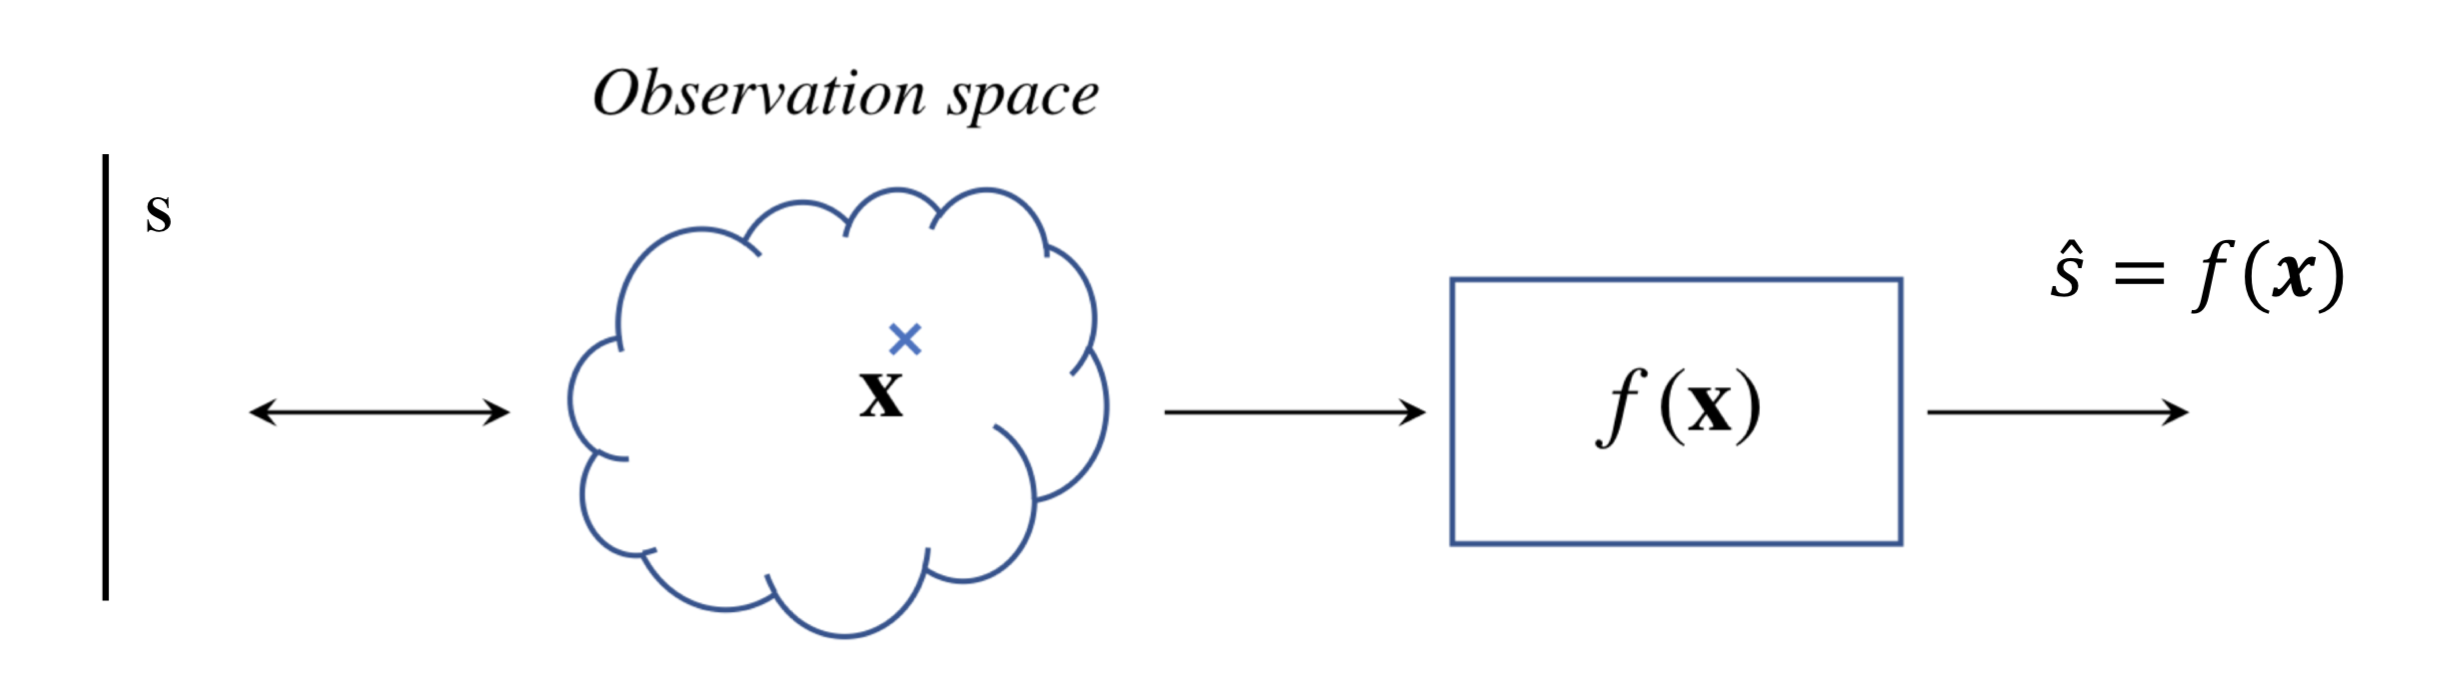
\includegraphics[width=10cm]{Figures//estimation_overview.png}
\end{center}
\caption{Diagram block of estimation problems.\label{fig:est_overview}}
\end{figure}

The estimation module applies a real output function $f(\cdot)$ that is commonly referred to as the \textit{estimator}, and its output, $\hat{S} = f(\mathbf{X})$, as the \textit{estimation} or \textit{prediction}. The estimator is a deterministic function, meaning that for a given value $\mathbf{x}$, it will consistently produce the same output. Although $f(\cdot)$ is deterministic if the input $\mathbf{X}$ is a random vector, the prediction $\hat{S}$ is a random variable.

The estimator is likely to incur some estimation error that will be quantified by means of a cost (or, alternatively, a reward) function. Designing our estimator will require minimizing (or maximizing) the expected value of this cost (reward).

We identify two main types of problems related to estimation:
\begin{itemize}
\item Analysis of estimators: given an estimator, evaluate its performance using a specific measure (a cost or a reward function).
\item Design of estimators: find a function $f(\mathbf{x})$ that optimizes a predefined goal.
\end{itemize}


%%%%%%%%%%%%%%%%%%%%%%%%%%%%%%%%%%%%%%%%%%%%%%%%%%%%%%%%%%%%%%%%%%%%
\subsection{Statistical information involved in estimation problems}
\label{subsec:statistical_info}

The statistical relation between the observations and the target variable is described by the {\bf joint} probability density function (pdf) of ${\bf X}$ and $S$: $p_{{\bf X},S}({\bf x},s)$, or some distribution related to it. 

The joint pdf can be factorized as products of conditional and marginal pdfs:
\begin{align}
p_{{\bf X},S}({\bf x},s) = p_{{\bf X}| S}({\bf x}| s) \cdot p_S(s) 
                         = p_{S|{\bf X}}(s|{\bf x}) \cdot p_{\bf X}({\bf x}) 
\end{align}

In the context of estimation theory, these factors receive specific names:

%%%%%%%%%%%%%%%
\begin{itemize}
\item The {\bf likelihood} of $S=s$ for observation ${\bf x}$, $p_{{\bf X}|S}({\bf x}|s)$: it characterizes the generation of observations for each value of the target variable.
\item The {\bf prior (or \textit{a priori}) distribution}  of $S$, $p_S(s)$: it describes how much is known (or unknown) about the target variable before observing ${\bf X}$. 
\item The {\bf posterior (or \textit{a posteriori}) distribution} of $S$ given ${\bf X}={\bf x}$, $p_{S|{\bf X}}(s|{\bf x})$: it describes the knowledge (or the uncertainty) about $S$ after observing ${\bf X}$.
% In the case where the variable to be estimated is deterministic, it does not make sense to condition the probability distribution of the observations to the value of $s$, so the strictly correct thing would be to denote the probability density of the observations simply as $p_{\bf X}({\bf x})$. However, note that for the estimation problem to make sense, the probability density of ${\bf X}$ has to be different depending on the real value of the deterministic parameter. For this reason, we will sometimes abuse notation and denote that dependence on observations with $s$ as $p_{{\bf X}|s}({\bf x}|s)$, referring to that probability density as the plausibility of $s$.
%\item {\bf Joint distribution} of ${\bf X}$ and $S$: $p_{{\bf X},S}({\bf x},s) = p_{{\bf X}|S}({\bf x}|s) p_S(s)$. It provides the most complete statistical modeling of the joint behavior of $\bf X$ and $S$.
\item The {\bf evidence} or marginal distribution of ${\bf X}$, $p_{{\bf X}}({\bf x})$.
\end{itemize}

%%%%%%%%%%%%%

The information available to design the estimator may depend on the application. A typical scenario, because it is related to the physical generative process of the observations, is the one in which the likelihood function is known, and the design of the estimator is based on it. If additionally, a prior distribution is available, the design can be grounded on the posterior distribution $p_{S|{\bf X}}(s|{\bf x})$, which can be calculated by means of Bayes' Theorem,
\begin{equation}
p_{S|{\bf X}}(s|{\bf x}) 
	= \frac{p_{{\bf X},S}({\bf x},s)} {p_{\bf X}({\bf x})} 
	= \frac{p_{{\bf X}|S}({\bf x}|s) p_S(s)}
	       {\int p_{{\bf X}|S}({\bf x}|s') p_S(s') ds'}
\end{equation}


%%%%%%%%%%%%%%%%%%%%%%%%%%%%%%%%%%%%%%%%%%%%%%%%%%%
\subsection{Cost functions for estimation problems}
\label{subsec_funcion_coste}

The evaluation and design of an estimator require some objective criteria. In some cases, we will consider that this criterion materializes in the form of a {\bf cost function} whose value we seek to minimize. %We note, however, that there are design strategies that fall outside of this approach, such as the direct maximization of some probability function.

A cost function $c(s,\hat s)$ is any measure of the discrepancy between the target variable and the estimation. It is generally non-negative, $c(s,\hat s) \geq 0$, with equality for $s = \hat s$. In some cases, the cost function can be expressed as a function of the estimation error $e= s-\hat s$ and we will write\footnote{Note that the cost function is denoted with a lowercase letter, $c$, because it is a deterministic function, i.e., for fixed values of $s$ and $\hat s$ the cost always takes the same value. However, as with the estimation function, the application of that function to random variables will result in another random variable, i.e., $C = c(S,\hat S)$.} $c(s,\hat s) = c(s - \hat s) = c(e)$. Some frequently used cost functions are:
\begin{itemize}
\item Quadratic cost: $c(e) = e^2$.
\item Absolute value of the error: $c(e) = |e|$.
\item Relative quadratic error: $c(s,\hat s) = \frac{(s-\hat{s})^2}{s^2}$
\item Cross Entropy: $c(s,\hat s) = - s \ln \hat s - (1-s) \ln (1-\hat s)$, for $s,\hat{s}\in [0,1]$
\end{itemize}

Since the target variable is unknown, the prediction cannot be computed by directly minimising the cost $c(s, \hat s)$, and we have to work with expectations. The expected value of the cost is usually referred as the {\bf risk} of an estimator $\hat{s}=f({\bf x})$:
\begin{align}
\label{Est:coste_medio_gen}
R_f = \EE\{c(S,\hat S)\} 
    & = \int_{\bf x} \int_s c(s,f({\bf x})) p_{S,{\bf X}}(s,{\bf x}) ds d{\bf x}
\end{align}
By the Law of Large Numbers, this is the average cost we can expect from a given estimator, after a large number of predictions.

The {\bf conditional risk} is the conditional mean for a given observation
\begin{align}
\label{Est:cond_risk}
R(\hat s, {\bf x}) = \EE\{c(S, \hat s) |{\bf x}\} 
           & = \int_s c(s,\hat s) p_{S|{\bf X}}(s|{\bf x}) ds
\end{align}


%%%%%%%%%%%%%%%
\begin{example}[Evaluation of estimators 1]
\label{CalculoECM}
Given the joint distribution
\begin{equation}
p_{S,X}(s,x) = \left[
\begin{array}{ll}
\frac{1}{x}, & \qquad 0 \le s \le x ~~{\rm and}~ 0 < x \le 1 \\
0,           & \qquad \text{otherwise}
\end{array}
\right.,
\end{equation}
consider the estimators $\hat{S}_1 = \frac{1}{2}X$ and $\hat{S}_2 = X$. Which is the best estimator from the point of view of the quadratic cost? To find out, we'll calculate the mean quadratic error for both estimators.
Knowing that, for any $w$,
\begin{align}
\mathbb{E}\{(S-wX)^2\}   
 &= \int_0^1 \int_0^x (s-wx)^2 p_{S,X}(s,x) ds dx   
  = \int_0^1 \int_0^x (s-wx)^2 \frac{1}{x}ds dx   \nonumber\\
 &= \int_0^1 \left(\frac{1}{3} - w  + w^2 \right) x^2 dx  
  = \frac{1}{3}\left(\frac{1}{3} - w  + w^2 \right) 
\end{align}
Taking $w=1/2$ and $w=1$ we get, respectively,
\begin{align}
\EE\left\{(S-\hat{S}_1)^2\right\} 
	&= \EE\left\{\left(S-\frac12 X\right)^2\right\}   
     = \frac{1}{3}\left(\frac{1}{3} - \frac{1}{2}  + \frac{1}{4} \right)
     = \frac{1}{36} \\
\mathbb{E}\{(S-\hat{S}_2)^2\} & = \mathbb{E}\{(S-X)^2\}   
 = \frac{1}{3}\left(\frac{1}{3} - 1  + 1 \right) = \frac{1}{9}
\end{align}
Therefore, from the point of view of the square error, $\hat{S}_1$ is a better estimator than $\hat{S}_2$.
\end{example} \vspace{0.2cm}
%%%%%%%%%%%%%


\begin{example}[Evaluation of estimators 2]
Assume that $S$ is a random variable of mean 0 and variance 1, and $X$ is a noisy observation of $S$,
\begin{equation}
X = S + R
\end{equation}
where $R$ is a random Gaussian variable, independent of $S$, of mean $0$ variance $v$. We will compute the risk for the estimator $\hat{S} = X$ and different cost functions. For the quadratic error:
\begin{equation}
\mathbb{E}\{(S-\hat{S})^2\} = \mathbb{E}\{(S-X)^2\} = \mathbb{E}\{R^2\} = v
\end{equation}
For the mean absolute error
\begin{align}
\mathbb{E}\{|S-\hat{S}|\}
    &= \mathbb{E}\{|R|\} 
     = \int_{-\infty}^{\infty} |r| \frac{1}{\sqrt{2\pi v}}\exp\left(-\frac{r^2}{2v}\right)dr 
\nonumber\\
    &= 2 \int_{0}^{\infty} r \frac{1}{\sqrt{2\pi v}}\exp\left(-\frac{r^2}{2v}\right)dr 
     = \sqrt{\frac{2v}{\pi}}
\end{align}
\end{example}\vspace{0.4cm}


%%%%%%%%%%%%%%%%%%%%%%%%%%%%%%
\subsection{Bias and variance}
\label{subsec_funcion_coste}

The bias of estimator $\hat S$ for a true target $S=s$ is defined as
\begin{align}
B(s) = \EE\{\hat S|S=s\} - s
\end{align}
and it accounts for the expected deviation of the estimator from the true value of the target variable.

\textcolor{magenta}{Note that, in general, the variance depends on the target. If a prior model for $S$, is available, we can compute the expected value to get
\begin{align}
B = \EE\{B(S)\} = \EE\{\hat S\} - \EE\{S\}
\end{align}}

The variance of estimator $\hat S$ for a true target $S=s$ is defined as
\begin{align}
V = \text{var}\{\hat S|S=s\} 
\end{align}
The variance accounts for the spread of the sampling distribution, or in other words, it quantifies how much the estimates vary from one sample ${\bf x}$ to another, for the same realization of $S$. Unlike bias, which assesses systematic deviation from the true parameter value, variance captures the randomness inherent in the estimation process due to sampling variability.


